%Template for PLoS
% Version 1.0 January 2009
%
% To compile to pdf, run:
% latex plos.template
% bibtex plos.template
% latex plos.template
% latex plos.template
% dvipdf plos.template
\documentclass[12pt]{article}

% amsmath package, useful for mathematical formulas
\usepackage[utf8]{inputenc}
\usepackage[T1]{fontenc}
\usepackage{amsmath}
\usepackage[mathlines,displaymath]{lineno}
\usepackage{mathtools}
% amssymb package, useful for mathematical symbols
\usepackage{amssymb}
\usepackage{natbib}
\usepackage[usenames,dvipsnames,table]{xcolor}
% graphicx package, useful for including eps and pdf graphics
% include graphics with the command \includegraphics
\usepackage{graphicx}
\usepackage{times}
\usepackage{tikz}
\usepackage{amsmath}
\usepackage{verbatim}
\usepackage{animate}
\usepackage{float}
\usepackage{boxedminipage}
\usepackage{color}
%\usepackage[portuguese]{babel}
\newcommand{\carlos}[1]{\textcolor{Red}{#1}}
\newcommand{\GM}[1]{\textcolor{Blue}{#1}}

\usetikzlibrary{arrows,shapes}

% cite package, to clean up citations in the main text. Do not remove.
%\usepackage{cite}

\usepackage{color} 

% package multirow for advanced formatting if tables
\usepackage{multirow}

% Use doublespacing - comment out for single spacing
%\usepackage{setspace} 
%\doublespacing


% Text layout
\topmargin 0.0cm
\oddsidemargin 0.5cm
\evensidemargin 0.5cm
\textwidth 16cm 
\textheight 20cm

% Bold the 'Figure #' in the caption and separate it with a period
% Captions will be left justified
\usepackage[labelfont=bf,labelsep=period,justification=raggedright]{caption}

% Remove brackets from numbering in List of References
\makeatletter
\renewcommand{\@biblabel}[1]{\quad#1.}
\makeatother

% Leave date blank
\date{}
%\doublespacing

\pagestyle{myheadings}

\begin{document}

\begin{flushleft}
{\Large
\textbf{Metacommunities in dynamic landscapes}
}
%% Insert Author names, affiliations and corresponding author email.
\\
\vspace{1.0cm} Charles N. de Santana$^{1,2,4,\ast}$, Jan
Klecka$^{1,3,\ast}$, Gian Marco Palamara$^{4}$, Carlos J. Meli\'an$^{1}$
\\
\vspace{1.0cm} \bf{1} Department of Fish Ecology and Evolution, EAWAG,
Swiss Federal Institute of Aquatic Science and Technology, Switzerland
\\
\bf{2} Programa de Pos-Graduaç\~{a}o em Ciencias da Terra e do Ambiente,
Universidade Estadual de Feira de Santana, Bahia, Brasil
\\
\bf{3} Laboratory of Theoretical Ecology, Institute of Entomology,
Biology Centre of the Academy of Sciences of the Czech Republic, Ceske
Budejovice, Czech Republic\\
\bf{4} Institute of Evolutionary Biology and Environmental Studies, University of Zurich, Switzerland\\
  \vspace{0.5 in}
  
  Keywords: patch dynamics, connectivity dynamics, seasonality,\\
  population dynamics, individual based model, random geometric networks,\\
  regional species richness, static landscapes, dynamic landscapes.\\
  Type of Article: Article\\
  Number of figures: 7 (5 in color); Number of tables: 2\\
$\ast$ Shared first authors\\
$\ast$ Corresponding author: charles.desantana@eawag.ch\\
\end{flushleft}

\newpage
% Please keep the abstract between 250 and 300 words
\section*{Abstract}
Predictions from theory and experiments have shown that high landscape connectivity promotes higher species richness than low connectivity. However, results demonstrating high diversity in low connected landscapes also exist. Whether landscape connectivity increases or decreases coexistence and species richness, factors driving landscape connectivity show intraday, seasonal or larger time scale variation \GM{I WOULD WRITE THE REMAINING PART OF THIS SENTENCE AS A NEW ONE: "The effects of fluctuations in landscape connectivity on species richness is lacking in metacommunity theory."} but their role to understand the effect of the fluctuations of landscape connectivity on species richness is lacking in metacommunity theory. Here we connect metacommunity dynamics to landscape dynamics in order to show that the amplitude and the frequency of landscape connectivity play a key role in predicting species richness. Our results show that regional species richness (i.e., $\gamma-$species richness) decays in static and low connected landscapes \GM{IS THIS ALREADY KNOWN IF YES WE SHOULD PUT SOMETHING LIKE: "confirming  classic result of metecommunity theory"}. For dynamic landscapes, $\gamma-$species richness also decays for low connected landscapes but only at high frequencies \GM{NOT SO CLEAR, ARE YOU MEANING: "We show a similar decay in species richness in dynamic landscapes that are characterized by high frequency of landscape connectivity"?}. Thus, $\gamma-$species richness is independent of how fragmented the landscape is for more than two order of magnitude frequency change \GM{OF WHAT?}. Furthermore, the fast decay in species richness as the landscape becomes fragmented in several components for static landscapes disappear in dynamic landscapes for a broad range of amplitude and frequency values driving landscape connectivity \GM{THE PREVIOUS SENTENCE IS NOT CLEAR AND TOO LONG. THE RESULT SHOULD BE EXPRESSED WITH 3 SENTENCES DESCRIBING THE MAIN FINDINGS}. Our results suggest that incorporating amplitude and frequency as determinants of landscape availability and connectivity together with patch dynamics into metacommunity theory promise significant advances in the field of metacommunity ecology and can provide new testable predictions of species diversity in fast changing landscapes.
\newpage
\section*{Introduction}

Metacommunity theory provides a number of insights into the role of dispersal for species coexistence in landscapes composed of units of suitable and unsuitable habitats. Theoretical and empirical studies have shown that different spatial processes can drive persistence and species richness (\cite{Holyoaketal2005}). Empirical studies have largely focused on dispersal rates with only recent emphasis on patterns of landscape connectivity (\cite{kneitel2004, cadotte2006}). Most results have shown that increasing connectivity tends to increase persistence and richness (\cite{ellneretal2001, foxetal2011}), but results showing a decrease in richness also exist (\cite{daviesetal2009, altermattetal2011}). Whether connectivity increases or decreases persistence and regional species richness, there are not yet predictions from metacommunity theory taking into account changes in landscape connectivity. Dispersal abilities of organisms, which define habitat connectivity, are affected by the fluctuations in the environment and various habitat characteristics (air temperature, moisture, currents and tides in aquatic environments, rainfall, landsliding, etc). Many of these factors fluctuate at different amplitudes and frequencies, with some showing high intraday variation while others fluctuate daily, seasonally or at larger time scales (figure 1). 

Landscape dynamics encompasses two major processes i.e., patch dynamics and variation in landscape connectivity. Patch dynamics, defined as changes of the number and position of patches, changes of patch habitat characteristics, size and suitability for a given species \GM{NOW PUT A NEW SENTENCE: "fluctuations in landscape connectivity is ... "}. Variation in habitat characteristics and landscape connectivity changing species richness and community structure may occur at all spatial and temporal scales. In some cases, the temporal and spatial scales are correlated; i.e. large-scale changes occur infrequently or slowly over a long time. Classic examples include gap dynamics in grasslands caused by animals (\cite{WhickerDetling1988, HobbsMooney1991, MiltonEtAl1997}), forest dynamics caused by individual tree-falls (\cite{Goldblum1997}) and larger-scale fires (\cite{VanWagnerEtAl2006, WhelanEtAl2013}) (figure 1). At larger temporal scales, transitions between habitat types at the continental scale occur during glacial-interglacial cycles (\cite{WerneckEtAl2011}). There are also examples of large-scale landscape dynamics over short
time scales, such as daily tides and seasonal changes of sea ice extent. These types of landscape dynamics may have profound implications for population dynamics of any kind of organism, from short to long lifespan. These fluctuations may also lead to different climate change velocities (\cite{loarieetal2009}), population divergence and speciation (\cite{aguileetal2011}), and changes of the latitudinal biodiversity gradient in deep time (\cite{mannionetal2014}).

\GM{NEW PARAGRAPH: "The joint effect of the amplitude and frequency of landscape connectivity on species richness has been rarely included in metacommunity studies." WHY THESE EFFECTS HAVE NOT BEEN STUDIED SO FAR? ADD ONE OR TWO SENTENCES WITH POSSIBLE REASONS.} Given the rapid changes observed in natural and human-disturbed landscapes, there is a growing need to develop methods that more accurately describe the effects of dynamic landscapes in metacommunities.

Patch dynamics, i.e. the process of destruction of patches and appearance of new ones has been addressed by numerous theoretical studies of metapopulations of single species. For example \cite{Hanski1999} derived formulas for predicting patch occupancy of a single population in landscapes with this type of patch dynamics. The mean species lifetime in a network of dynamical patches can also be estimated (\cite{DrechslerJohst2010}). Recent studies have shown that the rate of patch turnover is critical for metapopulation persistence. For example, \citet{reigadaetal2015} showed that increasing the rate of patch dynamics, i.e. patches are very ephemeral, decreases metapopulation persitence when dispersal is continuous, while persistence is facilitated by pulsed dispersal. 

\GM{NEW PARAGRAPH. "The links connecting different patches can also vary in time. For example ... ONE SENTENCE WITH EXAMPLES. Connectivity dynamics can therefore be critical in determining landscape structure. However connectivity dynamics has received little attention in metacommunity and metapopulation ecology (\cite{Holyoaketal2005}) ( WHY??). ANOTHER SENTENCE GIVING EXPLANATION. On the other hand, the concept of connectivity dynamics has been used in disease ecology (e.g. \cite{Ross2010}) (I WOULD CITE MORE THAN ONE STUDY). For example Seasonality in transmission rates can be described as a function of fluctuations of connectivity of the host .. etc (MORE CITATIONS)."} 

\GM{NEW PARAGRAPH} Despite the scarcity of theoretical predictions, there is a lot of empirical evidence that connectivity dynamics may play an important role \GM{IN WHAT?} but these studies have focused mostly in single metapopulation persistence. Connectivity is driven by the characteristics of the landscape matrix separating habitat patches (\cite{EycottEtAl2012}). For example, dispersal of amphibians between ponds is strongly affected by the terrestrial habitat separating the ponds (\cite{VanBuskirk2012, ClineHunter2014}), and by weather (e.g., moisture) (\cite{RittenhouseEtAl2009}). Dispersal of butteflies also depends on matrix environment (\cite{KueflerEtAl2010}) and dispersal kernels fluctuate in time (\cite{SchtickzelleEtAl2012}). In fish, interconnections between rivers forming during periods of heavy rain can connect otherwise disconnected habitats and allow for dispersal and gene flow (\cite{BoizardEtAl2009}). At larger spatial scales, connectivity of habitat patches in the polar regions fluctuates seasonally according to the extent of sea ice (figure 1 and animations SI-A1 and SI-A2). 

Patch and connectivity dynamics often act together to determine habitat and landscape availability for organisms with different dispersal abilities (\cite{LauranceEtAl1997, Hanski1999, DebinskiHolt2000, KattwinkelEtAl2009, MetzgerEtAl2009}). Wetlands are a good example where changes in patch size caused by varying precipitations and complete loss of some patches in the periods of drought drive strong seasonal fluctuations of landscape connectivity (\cite{RoshierEtAl2008, RuizEtAl2014}).\GM{THE NEXT SENTENCE IS TOO LONG AND NOT SO CLEAR TO ME} Large body of research in landscape ecology focused on the role of habitat conversion (e.g.,
forests turned into field or pastures etc.) and fragmentation \GM{OF WHAT?} predicts that habitat loss and fragmentation lead to a threshold beyond which there is a rapid species extinction (\cite{fahrig2002,ovaskainenhanski2003,rybickihanski2013}). These
studies mostly focus on a directed change in landscape structure, such as a transition from a continuous forest, to more isolated and smaller fragments of the original habitat (\cite{LauranceEtAl1997, MetzgerEtAl2009}). In this case, habitat destruction increases the distance between remaining patches which decreases landscape connectivity and disrupts dispersal of organisms. Apart from such directional changes, fluctuations in landscape availability (random or seasonal) are also common in nature (\cite{Sprugel1991, RuizEtAl2014}) (see figure 1) but their consequences for species richness received less attention, with the exception of disturbances (\cite{Sousa1984, SuppErnest2014}).

Here, we study the effect of amplitude and frequency \GM{OF WHAT?} on dispersal as determinants of landscape connectivity to explore their effect on regional species richness. Figure 1 illustrates the range of temporal and spatial scales that can be studied using the amplitude and frequency \GM{OF WHAT?} as determinants of landscape connectivity. We first aim to identify gaps in our knowledge of the patch and connectivity dynamics as the mechanisms driving species diversity in metacommunities (figure 2, table 1 for a glossary of main concepts, and figure SI-B1 for a summary of metapopulation and metacommunity studies). We then describe in detail our approach to explore the role of amplitude and frequency \GM{OF WHAT?} on the dispersal distances and their effect on landscape connectivity and regional species diversity (table 2 and figures 3-4). We explore two scenarios of landscape connectivity. \GM{YOU CANNOT MOVE DIRECTLY FROM AMPLITUDE AND FREQUENCY (A-F) TO MEAN AND VARIANCE (M-V) OF LANDSCAPE CONNECTIVITY. YOU SHOULD EITHER USE ALWAYS USE A-F OR ADD A SENTENCE WHERE YOU CLEARLY EXPLAIN HOW A-F IS RELATED TO M-V. FOR EXAMPLE "Any fluctuating signal with a given amplitude and frequency can be described using its mean and variance. For example a perfectly sinusoidal signal, measured along an integer number of periods, will have a variance proportional to the amplitude of the signal (see figure) and a mean on $\pi$."} The first scenario assumes the mean and the variance of landscape connectivity are dependent on each other (figure 3). The correlation for the mean and the variance is well established for some environmental factors and traits that follow Poisson process (e.g. the number of seeds or breeding events) and binomial process (e.g. presence--absence of flowers or proportion of seeds that germinate). In a Poisson-distributed trait, the mean equals the variance so that examining its variance is just as good as examining its mean (\cite{Nakagawal&Schielzeth2012}). The second scenario assumes that the mean and the variance in the factors changing landscape connectivity are independent of each other (\cite{Violletal2012}) (figure 3). We compare predictions from these two scenarios with fluctuating connectivity with static landscapes where connectivity is constant (figures 5-7). Finally, we propose a roadmap for incorporating landscape dynamics more realistically into metacommunity models.

Our results show that the number of species coexisting strongly differ between static and dynamic landscapes. While the mean $\gamma-$species richness decays in static and dynamic landscapes as the landscape becomes more and more fragmented, the variance in $\gamma-$species richness increases for more than two order of magnitude frequency change in dynamic landscapes \GM{IT IS NOT CLEAR WHAT YOU MEAN WITH "two order of magnitude frequency change in dynamic landscapes"}. This means that high or low $\gamma-$species richness can occur in dynamic landscapes for a broad set of amplitude and frequency values determining landscape connectivity. \GM{THE NEXT SENTENCE IS TOO LONG AND SO CLEAR TO ME} We also show that a fragmentation threshold which rapidly decreases species richness in static landscapes as well as in landscapes with coupled mean and variance of connectivity fluctuations disappears in dynamic landscapes for a broad set of amplitude and frequency values. These results suggest that species richness and the number of extinctions strongly depend of factors driving the mean and the variance of the dispersal threshold to connect two patches in the landscape. Our results suggest that connecting the mechanisms that drive changes \GM{AGAIN HERE YOU MOVE FROM M-V TO A-F. YOU SHOULD THEN PUT ANOTHER SENTENCE THAT MAKES THE CONNECTION BACK FROM M-V TO A-F} in amplitude and frequency \GM{OF WHAT?} to the determinants of patch dynamics into metacommunity models promise significant advances in the field of metacommunity ecology and can provide new testable predictions of species diversity in fast changing landscapes.

\section*{The model and its implementation}

In this section, we describe the computational model, while the
mathematical equations and further technical details are represented
in the online supporting information (SI-C). The mathematical
definitions are represented in table 2.

\subsection*{Static and dynamic landscapes}

We use a spatially explicit individual-based model in patchy and
dynamic landscapes. We run our simulations in landscapes consisting of
randomly located sites with range values between [0,1] representing
the universe of landscapes of any possible scale. Each patch $i$ has a
spatial location given by the coordinates $(x_{i}, y_{i})$. Two
patches $i$ and $j$ are connected by individuals dispersing if their
geographic distance, $\mathfrak{d_{ij}}$, is equal or smaller than a
critical threshold distance (i.e., dispersal radius),
$\mathfrak{d_{c}}$. This dispersal radius is fixed in static
landscapes and it follows a sinusoid function (i.e., seasonal
landscape) in dynamic ones. Dispersal radius to connect patch $i$ and
$j$ follows

\begin{equation}
\mathfrak{d_{c}} = \mathfrak{d_{0}} + \mathcal{A} sin (\pi \mathfrak{f} t),
\label{eq:ratioAf}
\end{equation}

with $\mathfrak{d_{0}}$, $\mathcal{A}$, $\mathfrak{f}$, and $t$ the initial
dispersal radius, the amplitude, the frequency, and time respectively. In
figure \ref{fig:Figure3} we show a graphical representation of how these
parameters change the dispersal radius and figure \ref{fig:Figure4} illustrates three possible landscapes to visualize the effect of the amplitude and frequency on the dispersal radius and landscape
connectivity (i.e., the number of connections of each patch $i$ with other sites in
the network changes with time, see animation SI-A3). In static landscapes, the
connectivity of the landscape is only a function of the initial dispersal
radius, $\mathfrak{d_{0}}$. As the ``static'' landscape name suggests, the
initial dispersal radius is the only value determining the threshold to connect
two patches. There is no variance related to this initial dispersal radius
value, and thus there is a fixed dispersal radius given by $\mathfrak{d_{c}} =
\mathfrak{d_{0}}$.

In dynamic landscapes the amplitude and frequency values
together with the initial dispersal radius determine the dispersal
radius and the connectivity of the landscape. Thus, the amplitude and frequency
values add a variance to the initial dispersal radius, $\mathfrak{d_{0}}$. The simplest scenario
would be to assume that the initial dispersal radius is equal to the
amplitude of the fluctuations of the dispersal radius (i.e.,
$\mathcal{A} = \mathfrak{d_{0}}$). In this scenario, the mean and the
variance of the dispersal radius and landscape connectivity are not
independent of each other. We call this scenario coupled dynamic
landscape because factors producing a low (or high) mean dispersal
radius also produce a low (or high) variance (figure \ref{fig:Figure3}). There may be
situations, however, where the mean and the variance in the factors
changing landscape structure are independent of each other
(\cite{Violletal2012}). In order to account for the independence between the mean and the variance in landscape connectivity, we explore a scenario where the initial mean dispersal radius is
independent of the amplitude values (i.e., $\mathcal{A} \neq
\mathfrak{d_{0}}$). We call this general scenario "dynamic landscape", with the "coupled dynamic landscape" (i.e., $\mathcal{A} = \mathfrak{d_{0}}$) being a special case.

\subsection*{Population dynamics and dispersal in dynamic landscapes}

In ouir approach there can be several species in each patch and the state of each patch is described by a vector with abundance values for each species. To model spatio-temporal changes in the abundance of these patches, we need to
define dispersal rules together with population dynamics. We assume that all patches are of the same size and habitat type; we do not associate a priori a value for each patch which determines the habitat type as, for example, \cite{rybickihanski2013} do. Instead, we allow individuals to disperse between any two patches only as a
function of species abundance of the leaving patch. In this scenario
individuals only can move between connected $i$ and $j$ patches (i.e., those patches
satisfying the condition $\mathfrak{d_{ij}}$ $\leq$
$\mathfrak{d_{c}}$). At the beginning of the simulations we have an
initial population that spreads instantaneously across the whole
landscape. We assume that all patches are fully occupied and have the
same carrying capacity, i.e., population size at a given patch $i$,
$J_{x_i,y_i}$, is equal to the patch environmental carrying
capacity. The total number of individuals in the landscape is $J$ =
$J_{x_1,y_1}$ + $J_{x_2,y_2}$ + $J_{x_3,y_3}$ + $J_{x_4,y_4}$,..., +
$J_{x_\mathcal{P},y_\mathcal{P}}$, with $\mathcal{P}$ the total number
of patches.

Population dynamics on the spatial network occur under a zero-sum birth and
death process in overlapping generations. This means that at each time step an
individual dies from a randomly chosen patch {\em i}. This individual is
replaced with an individual coming from another patch (i.e., migrant), from the
same patch than the death individual or from the regional species pool. Parents
are chosen with probability $m$ from outside patch {\em i} within the network,
with probability $\nu$ from the regional species pool, or with probability
$\lambda$ (i.e. local birth rate), defined as $\lambda$ = $1 - m - \nu$, from
the patch {\em i}. We consider an extremely diverse regional species pool
containing an infinite number of species. Because of the infinite number of
species in the regional pool, we assume that every immigration event introduces
a new species. Immigration of a new species corresponds to speciation in the
context of metacommunity models \citep{Vanpeteghem&Haegeman:2010}. The
dispersal from patch $j$ to patch $i$ of species $k$ is defined by:

\begin{equation}
  m_{ij}^{k} =  \frac{m}{\mathfrak{d_{ij}}},
\label{neutdis}
\end{equation}
with $\mathfrak{d_{ij}}$ the geographical distance between patch $i$
and $j$ satisfying $\mathfrak{d_{ij}}$ $\leq$ $\mathfrak{d_{c}}$ and
$m$ is the intensity of emigration rate. Because dispersal from patch
$i$ to patch $j$ is the same as in the opposite direction
($m_{ji}^{k_{\phi}} = m_{ij}^{k_{\phi}}$), this represents symmetric, patch- and density-independent dispersal where dispersal to connected and less distant patches is more likely than dispersal to more
distant patches.

\subsection*{Implementation and simulations}

Prior to the simulations, one needs to specify the parameters for
generating the landscape and the regional pool of species. The
landscape is generated following a 2D-random geometric network as
described in the section ``Static and dynamic
landscapes''. Simulations were carried out with an initial population
at each patch $i$, $J_{x_i,y_i}$, of 100 individuals for a total of
100 patches. The population size and the number of patches remained
constant throughout the simulations. Results for figures 5-7, SI-D1 and SI-E1 were obtained after 100 replicates with 1000 generations each, where a generation, $\mathcal{G}$, is an update of the total number of individuals, $J$, in the landscape. Values plotted represent the mean and the variance
across the last 500 generations per replicate. We explored a broad range of parameter values
from a uniform distribution with values $\mathcal{U}[0.001,1]$ for the
initial dispersal radius, $\mathfrak{d_{0}}$, the amplitude,
$\mathcal{A}$, and the frequency, $\mathfrak{f}$. We set mortality
rates equal to 1 (i.e., the natural mortality rate, $\mu$). Rates of
immigration from the regional species pool, $\nu$, and the intensity
of emigration rate, $m$, were set to 0.003, and
0.1, respectively. Local birth rates for each metacommunity,
$\lambda = 1 - \nu - m$, so that a new individual replacing the dead
individual appears with certainty.

\subsection*{Landscape connectivity and $\gamma-$species richness}

We calculated the mean number of components per replicate as a proxy of landscape connectivity and availability (see SI-D1) together with the mean and variance regional species richness (i.e., $\gamma-$species richness) for the simulations with
static and dynamic landscapes. A component can be formed by one or several isolated patches. We plotted the mean and variance
$\gamma-$species richness vs. all amplitude ($\mathcal{A}$), frequency ($\mathfrak{f}$), and dispersal radius ($\mathfrak{d_{0}}$) values explored (figures 5-7 and SI-E1). 

\section*{Results}

Mean regional species richness (i.e., mean $\gamma-$species richness) decays for static and dynamic landscapes for a broad range of amplitude and frequency values (figure 5, top). Variation in the frequency values that alter the dispersal radius to connect each two patches has strong implications for the dynamics of $\gamma-$species richness. While the variance in $\gamma-$species richness has the same behavior than the mean for static landscapes (figure 5, bottom left), it changes its behavior for dynamic landscapes (figure 5, bottom right). The variance of $\gamma-$species richness also decreases for high frequency values (figure 5, bottom right, red, orange and yellow circles, $\mathfrak{f}$ $\geq$ 0.1), but the opposite occurs for low values (figure 5, bottom right, green, light blue and blue circles, $\mathfrak{f}$ < 0.1). Thus, $\gamma-$species richness is independent of how fragmented the landscape is for two order of magnitude frequency change ($\mathfrak{f}$ = [0.001,0.1], \carlos{P-VALUES AND $R^2$ FOR EACH FREQUENCY: HOW MANY FREQUENCIES DO HAVE NON-SIGNIFICANT RELATIONSHIP?}). For low frequency values, largely fragmented landscapes (i.e., high number of components) can have high or low regional species richness and the prediction of lower richness with more fragments (or viceversa) is broken. We have obtained similar $\gamma-$species richness values for all the amplitude, $\mathcal{A}$, and frequency, $\mathfrak{f}$, values explored for all the landscape metrics used and for the analysis presented here we have used the mean number of components as a proxy of landscape connectivity (figure SI-D1).

Our analysis show a landscape fragmentation threshold which rapidly reduces $\gamma-$species richness in static landscapes as well as in landscapes with coupled mean and variance of connectivity fluctuations (figures 6-7 and SI-E1). Increasing the dispersal radius rapidly recovers landscape connectivity and $\gamma-$species richness in static (figure 6, top left) and for high frequency values in dynamic landscapes (figure 6, top right for frequency values in red, orange and yellow circles, $\mathfrak{f}$ $\geq$ 0.1). This rapid decay in landscape connectivity and species richness can also be visualized in figure 7 and follows from the predicted analytical percolation threshold in random geometric graphs \carlos{REFERENCE HERE OR EXPLAINED IN THE PREVIOUS SECTION}. The critical threshold in our landscape is given by $D_c$ = $L$ $\times$ sqrt(4.52/(4 $\times$$\pi$ $\times$$\mathcal{P}$)) = 0.06 (figure 7, dotted line, log10(0.06) = -1.22), where $L$ is 1, and $\mathcal{P}$ the number of patches, 100 (\carlos{WE ALSO NEED TO ADD THE BLACK LINE TO FIGURE 6}). This critical threshold reducing $\gamma-$species richness in static landscapes disappear in dynamic landscapes (figures 6, top right, 7 and SI-E1). The threshold is less strong when considering the variance in $\gamma-$species richness for the static landscape (figure 6 bottom left) and it completely disappears for several frequency values in dynamic landscapes (figure 6, bottom right). 

To explore the robustness of the changes of $\gamma-$species richness in static, coupled dynamic, and dynamic landscapes we explored a broad range of amplitude, frequency and dispersal radius values (figure 7 and SI-E1). Predictions of $\gamma-$species richness under coupled dynamic landscapes (i.e., the mean and the variance in the factors changing landscape connectivity are dependent of each other) follow qualitatively the same results as the ones predicted by the static landscapes (compare blue and black lines, figure 7). These results are robust for three order of frequency change (figure SI-E1 for frequency, $\mathfrak{f}$ = 0.001 (a), 0.01 (b), 0.1 (c) and 1 (d)). The critical threshold reducing $\gamma-$species richness in static and coupled dynamic landscapes disappears in dynamic landscapes for two order of magnitude change in frequency values (figure SI-E1 for frequency, $\mathfrak{f}$ = 0.001 (a), 0.01 (b), 0.1 (c)). We remark these results were obtained using intensity of emigration values of 0.1. They represent a conservative estimation because larger intensity of emigration values may predict a stronger removal of the critical threshold for dynamic landscapes and a larger difference between the predicted $\gamma-$species richness for the dynamic and the static landscapes the than the ones reported here (\carlos{SHOULD WE REPORT A FIGURE WITH M = 0.3 TO SHOW A STRONGER ELIMINATION OF THE THRESHOLD FOR DYNAMIC LANDSCAPES?}). In summary, our results for the regional species richness from static, coupled dynamic and dynamic landscape strongly differ for a broad range of amplitude, $\mathcal{A}$, and frequency, $\mathfrak{f}$, values. The fast decay in species richness as the landscape becomes fragmented in static and coupled dynamic landscapes disappears in dynamic landscapes for a broad range of amplitude and frequency values.

\section*{Discussion}

Our study adds to previous attempts to connect species persistence to dynamic landscapes (\cite{Hanski1999,keymeretal2000}). Our goal was to understand how the many factors that drive landscape connectivity with some showing high intraday variation while others fluctuate daily, seasonally or at larger time scales can be captured by the amplitude and frequency of change in landscape connectivity and how the amplitude and frequency fluctuations determining landscape connectivity can drive coexistence in multispecies communities. Our results show that the number of species coexisting strongly differ between static and dynamic landscapes. While the $\gamma-$species richness decays in static and dynamic landscapes as the landscape becomes more and more fragmented, the variance in $\gamma-$species richness increases for a broad range of frequency change values (figures 5-7). This means that high or low $\gamma-$species richness can occur in dynamic landscapes for a broad range of amplitude and frequency determining landscape connectivity. Our results also show that a fragmentation threshold which rapidly decreases species richness in static landscapes as well as in landscapes with coupled mean and variance of connectivity fluctuations disappears is dynamic landscapes for a broad range of amplitude and frequency values. Thus,  $\gamma-$species richness is independent of how fragmented the landscape is for more than two order of magnitude frequency values (figure 5). These results suggest that largely fragmented landscapes (i.e., landscapes with a high number of components) can have high or low regional species richness. Our results suggest that fast changing frequencies in the landscape predict qualitatively the same outcomes than static landscapes, a result that may help to connect predictions from fast changing landscapes with analytical predictions obtained from the classical metacommunity theory in static landscapes (figures 5 and 6). Our results, however, also predict that there are a broad range of parameter combinations (more than two order of magnitude of amplitude and frequency change, figures 6 and 7) whose predictions strongly differ from the predictions under fast changing landscapes or static landscapes. New approximations are required to understand species richness and persistence for those dynamic landscapes. 

Larger landscape connectivity and migration rates tend to homogenize metacommunities and decrease species richness (\cite{ellneretal2001, foxetal2011}). Two examples are predator-prey systems and competing communities. High landscape connectivity in predator-prey systems tends to destabilize preys and decrease richness (\cite{ellneretal2001, foxetal2011}). Competitive communities with highly connected landscapes tend to have only a few dominant species (\cite{Holyoaketal2005}). How do the strength and direction of migration and habitat selection change the results presented in this study? Our approach did not explicitly test for directionality of migration or selection and we assumed equal growth rates across the landscape, nor did we assume any asymmetry in competition or trophic interactions as possible mechanisms for structuring diversity in our static and dynamic landscapes, hence a neutral theory of biodiversity in dynamic landscapes was applied. While our model assumes neutral dynamics and random geometric graphs for population fluctuations, we expect stronger differences than the ones found in this study between static and dynamic landscapes under more realistic scenarios. For example, in our model all the individuals and species use equally the available connections between patches and the continuity of the landscape but niche differences between species, different habitat preferences in the landscape or highly heterogeneous landscapes may produce different results about the percolation threshold for $\gamma-$species richness in dynamic landscapes. In our approach dynamic landscapes predicts higher regional species richness compared to static landscapes mostly because landscapes patches are alternately isolated and then highly connected for periods of time that can sustain more species than a static landscape with the same mean dispersal radius (patches moderately connected all the time). Tentative support for this prediction is provided by studies of river systems which show that even brief periods of increased connectivity may lead to gene flow with significant effects on genotypic diversity of populations over the landscape (\cite{BoizardEtAl2009}). In the metacommunity context, brief periods of high landscape connectivity may allow local species to spread rapidly to a number of new sites which provide opportunities for population growth and rescue from extinction by demographic stochasticity in small local populations. 

Microcosms experiments with contrasting regimes of amplitude and frequency determining connectivity fluctuations would be necessary to test our predictions under laboratory conditions. Model systems like bacteria, protists (\cite{Carrara2012dendritic}), small invertebrates such as zooplankton (\cite{Steiner2011seasonal_experiments}) or insects (\cite{GovindanSwihart2012}) may provide a sufficient level of control over the landscape-level parameters to test predictions from dynamic landscapes models. Long-term data can also be used to explore landscape dynamics models incorporating more realistic climatic regimes or broader geographic regions in deep time to infer the amplitude and frequency (or additional parameters capturing fluctuations at different temporal scales) that best predict the spatio-temporal fluctuations in species diversity. For example, there is evidence of fast changing landscapes in the Arctic and Antarctic regions with the ice cover dynamics (animations SI-A1 and SI-A2), but the amplitude and frequency required to predict such fluctuations and their impact on local and regional species richness are currently unknown (\carlos{WE WOULD NEED TO CHECK SOME STUDIES HERE}). These approximations can also help to discern how much complexity is required to make predictions that fit periods of peaks or flattened species richness gradients as observed in the fossil record for some periods of the latitudinal biodiversity gradient (\cite{mannionetal2014}). In this situation, transitions between habitat types at the continental scale occur during glacial-interglacial cycles may combine with larger temporal scales that would require to include non periodic dynamic landscapes (i.e., plate tectonic or continental drift) (\cite{WerneckEtAl2011}).

 
\subsection*{Future perspectives}

Natural metacommunities are facing different types of dynamical changes. Patch dynamics has already received substantial attention but predictions from connectivity dynamics are still rare. Our results together with previous studies show that landscape dynamics may have important implications for species richness but the combined effect of patch and connectivity dynamics is still missing. Future research would need to combine patch and connectivity dynamics to further advance our understanding of short- and large-scale patterns of biodiversity dynamics. Adding a more realistic description of landscape dynamics into metacommunity models would necessarily increase their complexity and likely preclude analytical solutions. Here we have developed an individual-based model to explore the effect of amplitude and frequency on connectivity fluctuations and species richness but extending this approach by including patch dynamics is straightforward. For example, in addition to temporal fluctuations of dispersal radius (equation 1 and equations in SI-C), we can simulate destruction of patches and creation of new patches at random time points. Similarly, spatial heterogeneity or temporal fluctuations in the carrying capacity of individual patches could be included. We can thus start to explore the interactive effects of patch and connectivity dynamics on local and regional species richness. Empirical studies suggest that these interactive effects may have important effects on biodiversity (e.g. \cite{LauranceEtAl1997, RoshierEtAl2008, MetzgerEtAl2009, RuizEtAl2014}), but robust predictions from the theory and connections between the predictions and empirical data are still lacking. 

\section*{Acknowledgments}

This study was supported by the Swiss National Science Foundation
project 31003A-144162 (to C. deS. and C. M.) and by the Sciex fellowship
project 12.327 (to J. K.)

\newpage
%\section*{References}
% The bibtex filename
\bibliographystyle{ecol_let.bst}
\bibliography{references}

\restylefloat{table}
\section*{Tables}

\begin{table}[H]
\rowcolors{1}{white}{pink!20}
\begin{tabular}{  p{6cm}  |  p{10cm} }
  \hline
  \textbf{Concept} & \textbf{Explanation}\\  \hline
  Metapopulation & A set of local populations connected by dispersal which occupy discrete patches of suitable habitat embedded in a matrix of unsuitable environment \\ \hline
  Metacommunity &  An extension of the metapopulation concept to a multispecies setting; 
  i.e. a set of local communities connected by dispersal \\ \hline  
  Landscape dynamics & Changes in the number, position, and characteristics of habitat patches (patch dynamics) and connectivity fluctuations \\ \hline
  Patch dynamics & Changes in the number and position of habitat patches (i.e., destruction and creation of patches) and changes of habitat 
  characteristics of local patches (changes in vegetation type, abiotic conditions, etc) \\ \hline
  Connectivity dynamics & Changes in properties of the matrix organisms have to cross 
to disperse from one patch to another and changes in other external environmental conditions affecting dispersal \\ \hline
  Random geometric network  & A spatial network of patches connected by links if they are located within a defined dispersal radius \\ \hline
 Number of components & Number of isolated patches or group of patches in the landscape \\ \hline
  Dispersal radius  & Maximum distance between a pair of patches which allows dispersal between the patches (i.e., patches with larger distance are not connected) \\ \hline
   %Density-independent immigration  & Colonizing a patch is independent of species density. \\ \hline
  %Density-dependent mortality & Probability to die is a function of species density \\ \hline        
  %Density-dependent emigration & Probability to leave a patch is a function of species density \\ \hline
\end{tabular}
\label{table1}
\caption{Glossary of concepts}
\end{table}

\newpage
\begin{table}[h]
\rowcolors{1}{white}{pink!20}
\begin{tabular}{  p{5cm}  |  p{10cm} }
 \hline
  \textbf{Symbol} & \textbf{Concept}\\  \hline
  $J_{x_i,y_i}$ & Community size of patch $i$ with coordinates $x_i$ and $y_i$ \\ \hline
  $\mathcal{P}$ & Total number of patches \\ \hline
  $\mathfrak{d_{c}}$ = $\mathfrak{d_{0}} + \mathcal{A} sin (\pi \mathfrak{f} t)$ & Dispersal radius to connect two patches \\ \hline
  $\mathfrak{d_{0}}$ & Initial dispersal radius \\ \hline
  $\mathcal{A}$ & Amplitude of change in the dispersal radius \\ \hline
  $\mathfrak{f}$ & Frequency of change in the dispersal radius \\ \hline
  $\mathcal{G}$ & Generation time or complete turnover in the landscape \\ \hline
  $\mathfrak{d_{ij}}$ & Geographical distance between patch $i$ and $j$ \\ \hline
  %$\mathfrak{d_{c_{min}}}$ & Minimum distance between any pair of patches \\ \hline
  %$\mathfrak{d_{c_{max}}}$ & Maximum distance between any pair of patches \\ \hline
  %$\sigma^{2}$[$\mathfrak{d_{c}}$] & Variance radius to connect two patches 23. STANDARIZE SYMBOLS IN FIGURES \\ \hline
  $\Gamma_{i}$ = $\sum_{j \neq i} (\mathfrak{d_{ij}} < \mathfrak{d_{c}})$ & Connectivity patch $i$ \\ \hline
  $\mathrm{m}$ & Emigration rate \\ \hline
  $\mathrm{\nu}$ & Immigration rate from the regional species pool \\ \hline
  $\lambda$ & Local birth rate \\ \hline  $\mu$ & Local natural mortality \\ \hline
  $\mathrm{N^{k}_{i}}$ & Abundance of species $k$ in patch $i$ \\ \hline  
  %$\alpha$-richness & Number of species in patch $i$ \\ \hline
  $\gamma$-richness & Number of species in the landscape \\ \hline
  $\mathrm{m^{k}_{ij}}$ = ($\mathrm{m}$/$\mathfrak{d_{ij}}$)($\mathrm{N^{k}_{j}}$/$J_{x_j,y_j}$) & Dispersal from patch $j$ to $i$ for species $k$ with abundance $\mathrm{N^{k}_{j}}$ \\ \hline
  $\mathcal{C}$ & Number of components in the landscape \\ \hline
  $\hat{\mathcal{C}}$ & Mean number of components in the landscape  \\ \hline
  %Symmetric \vspace{0.01 in} dispersal & Dispersal probability between two sites is the same in both directions. \\ \hline
  %Density-independent \vspace{0.01 in} immigration (random) & Colonizing a site is not a function of the species density in the receiving site. \\ \hline
  %Density-dependent mortality & Probability to die is a function of species abundance. \\ \hline        
  %Density-dependent emigration & Probability to leave a site is a function of species abundance. \\ \hline
%  \bottomrule
\end{tabular}
\caption{Symbols used and definitions}
\label{table2}
\end{table}

\vspace{5 in}
\newpage

\section*{Figure Legends}

\noindent{Figure 1: Fluctuations in landscape connectivity and patch
  characteristics occur at many spatial and temporal scales. Spatial
  and temporal scale is often correlated (Blue ellipse). Seasonal and
  daily changes (e.g. tides) are prominent examples of fast processes
  happening across all spatial scales (Green ellipses). One example of
  the regional fluctuations between years in landscape connectivity is
  the ice-cover changes in the Artic and Antarctic regions (See
  animation SI-A1 and SI-A2, respectively). These fluctuations may be
  characterized by the amplitude, $\mathcal{A}$, and frequency,
  $\mathfrak{f}$, that combined determine the connectivity of the
  landscape. \carlos{WE HAVE TO BE A BIT MORE PRECISE IN THIS FIGURE. FOR EXAMPLE, WE HAVE TO PUT A LINE AND SOMETHING LIKE AN ERROR BAR AROUND THE PLATE TECTONIC AND CONTINENTAL DRIFT. WE ALSO SHOULD INTRODUCE CLASSICAL CYCLES LIKE THE MILANKOVITCH CYCLES: ECCENTRICITY (APPROX. BETWEEN 100,000-400,000 YEARS); OBLIQUITY (APPROX 41,000y), AND PRECESSION (APPROX 22,000y). THESE CYCLES ARE IMPORTANT TO DRIVE GLACIAR AND INTERGLACIAR PERIODS.}}

\noindent{Figure 2: Two major processes of landscape dynamics: 1. Patch dynamics represent changes of the number and position of patches, changes of patch habitat characteristics, size and suitability and 2. Connectivity dynamics may start with an identical landscape but changes in the landscape matrix produce different landscapes at future time points. Both dynamics, patch and connectivity dynamics, may happen at the same time.}}

\noindent{Figure 3: Dispersal radius to determine whether two patches are connected, $\mathfrak{d_{c}}$, is a function of the initial dispersal radius, $\mathfrak{d_{0}}$, amplitude, $\mathcal{A}$, and frequency, $\mathfrak{f}$. In static landscapes the dispersal radius is equal to the initial dispersal radius (i.e., $\mathfrak{d_{c}} = \mathfrak{d_{0}}$). In the coupled dynamic landscape scenario, the value of dispersal radius fluctuates around the mean dispersal radius, $\mathfrak{d_{0}}$ = $\mathcal{A}$, with 2$\mathcal{A}$ as the value of the maximum fluctuation, and the frequency, $\mathfrak{f}$, as
  the inverse of the period of the seasonal fluctuation. In the dynamic landscape scenario the initial dispersal radius, $\mathfrak{d_{0}}$, is independent of the amplitude, $\mathcal{A}$.}

\noindent{Figure 4: Landscape connectivity in three scenarios of low dispersal radius (a, $\mathfrak{d_{c}} = 0.01$), medium dispersal radius, (b, $\mathfrak{d_{c}} = 0.03$), and large dispersal radius, (c, $\mathfrak{d_{c}} = 0.075$). Two patches $i$ and $j$ are connected if their geographical distance, $\mathfrak{d_{ij}}$, is lower or equal than the dispersal radius, $\mathfrak{d_{c}}$.}

\noindent{Figure 5: This figure represents the mean (Top) and variance (Bottom) of $\gamma$-richness as a function of the mean number of components in the landscape (i.e., large number of components represents a low connected landscape). The lower the mean number of components of the landscape the higher is the mean $\gamma$-richness for both static (Top left) and dynamic (Top right) landscapes. The variance in $\gamma$-richness has the same behavior than the mean for static landscapes (Bottom left). The variance in $\gamma$-richness also decreases for high frequency values but not for low frequency values (Bottom right). Thus, for low frequency values $\gamma$-richness is independent of the number of components in the landscape. Circles represent the mean (Top) and the variance (Bottom) of $\gamma$-richness after the past 500 generations for each replicate. \carlos{FREQUENCY VALUES IN BAR}}

\noindent{Figure 6: This figure represents the mean (Top) and variance (Bottom) of $\gamma$-richness as a function of the dispersal radius (i.e., large dispersal radius increases connectivity in the landscape). There is a critical threshold for the dispersal radius in static landscapes where $\gamma$-richness decays nonlinearly (Top left). This threshold remains for high frequency values in dynamic landscapes (Top right), but not for low frequency values where we can have a large number of species for highly fragmented landscapes. Circles represent the mean (Top) and the variance (Bottom) of $\gamma$-richness after the past 500 generations for each replicate. \carlos{Bar representing the frequency values explored and the colors associated.}}

\noindent{Figure 7: (Top) Represents $\gamma-$species richness as a
  function of the initial dispersal radius, $\mathfrak{d_{c}}$, for static
  landscapes (black line, $\mathcal{A}$ = 0), coupled dynamic landscapes
  (blue line, $\mathcal{A}$ = $\mathfrak{d_{c}}$ and $\mathfrak{f}$ =
  0.01), and dynamic landscapes (red line, $\mathcal{A}$ = 1 and
  $\mathfrak{f}$ = 0.01). Vertical dotted line represents the critical
  threshold in static landscapes. (Bottom) $\gamma-$species richness as a function of the
  dispersal radius, $\mathfrak{d_{c}}$, and amplitude $\mathcal{A}$
  for frequency values, $\mathfrak{f}$ = 0.01. Isoclines (dotted
  lines) represent the mean number of components, $\hat{\mathcal{C}}$, for
  each combination of dispersal radius, $\mathfrak{d_{c}}$, and
  amplitude $\mathcal{A}$. Red, blue, and black lines represent
  dynamic, coupled dynamic and static landscapes, respectively, with
  the same values as in the top panel. Simulations were done for emigration
  rate, $\mathrm{m}$ = 0.1, immigration rate from the species regional
  pool, $\mathrm{\nu}$ = 0.003, total number of patches, $\mathcal{P}$
  = 100, patch size, $J_{x_i,y_i}$ = 100 individuals and number of
  generations per replicate, $\mathcal{G}$ = 1000. Species richness
  was averaged over the last 500 generations in each replicate.}


\newpage

\restylefloat{figure}
\section*{Figures}

\begin{figure}[hb!]
\hspace{-0.5 in}\includegraphics[width=6in]{./figures/Figure1.eps}
\caption{}
\label{fig:Figure1}
\end{figure}

\begin{figure}
\hspace{0.75 in}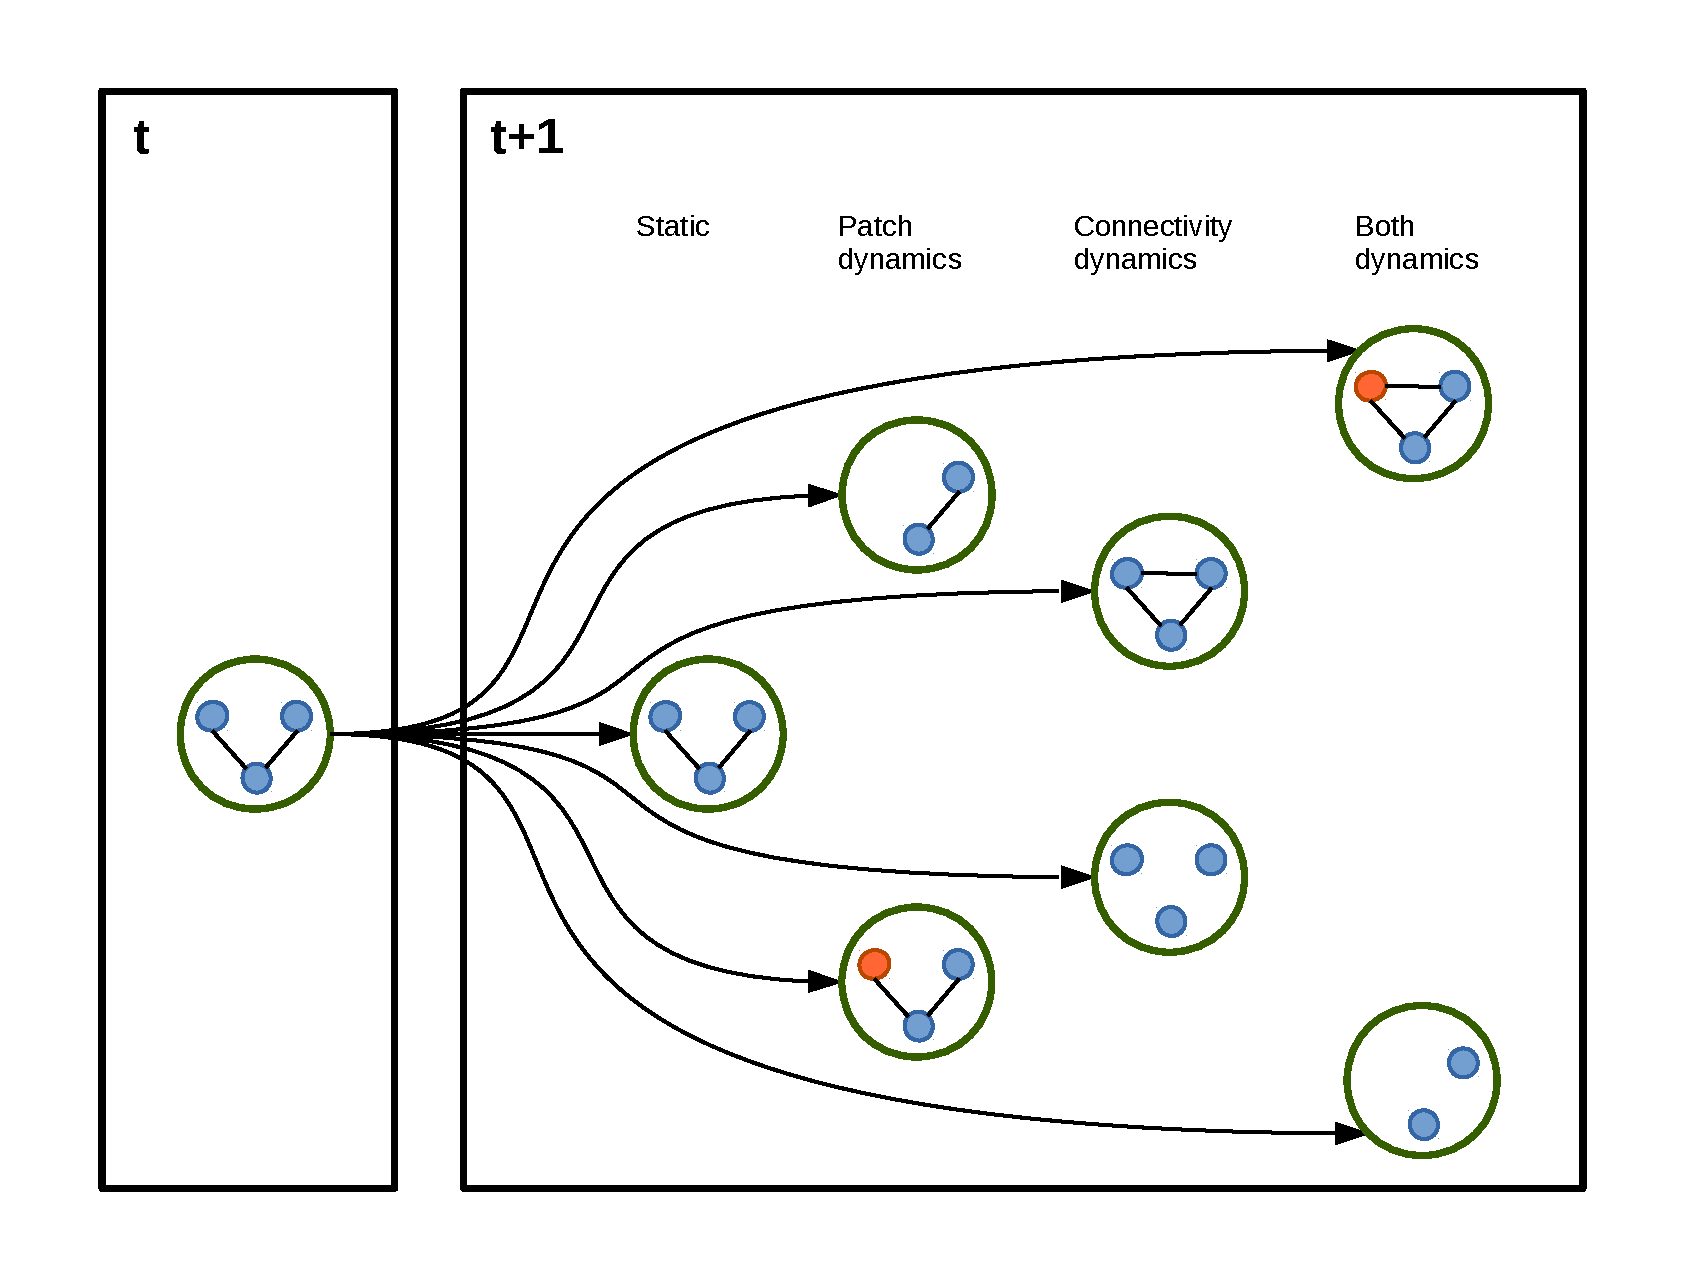
\includegraphics[height=4in,width=5in]{./figures/Figure2.eps}
\caption{}
\label{fig:Figure2}
\end{figure}

\begin{figure}[hb!]
%\begin{center}
\includegraphics[width=4in, angle=-90]{./figures/BasisForEquation.eps}
%\end{center}
\caption{}
\label{fig:Figure3}
\end{figure}

\begin{figure}[hb!]
\begin{center}
%\hspace{-0.5 in}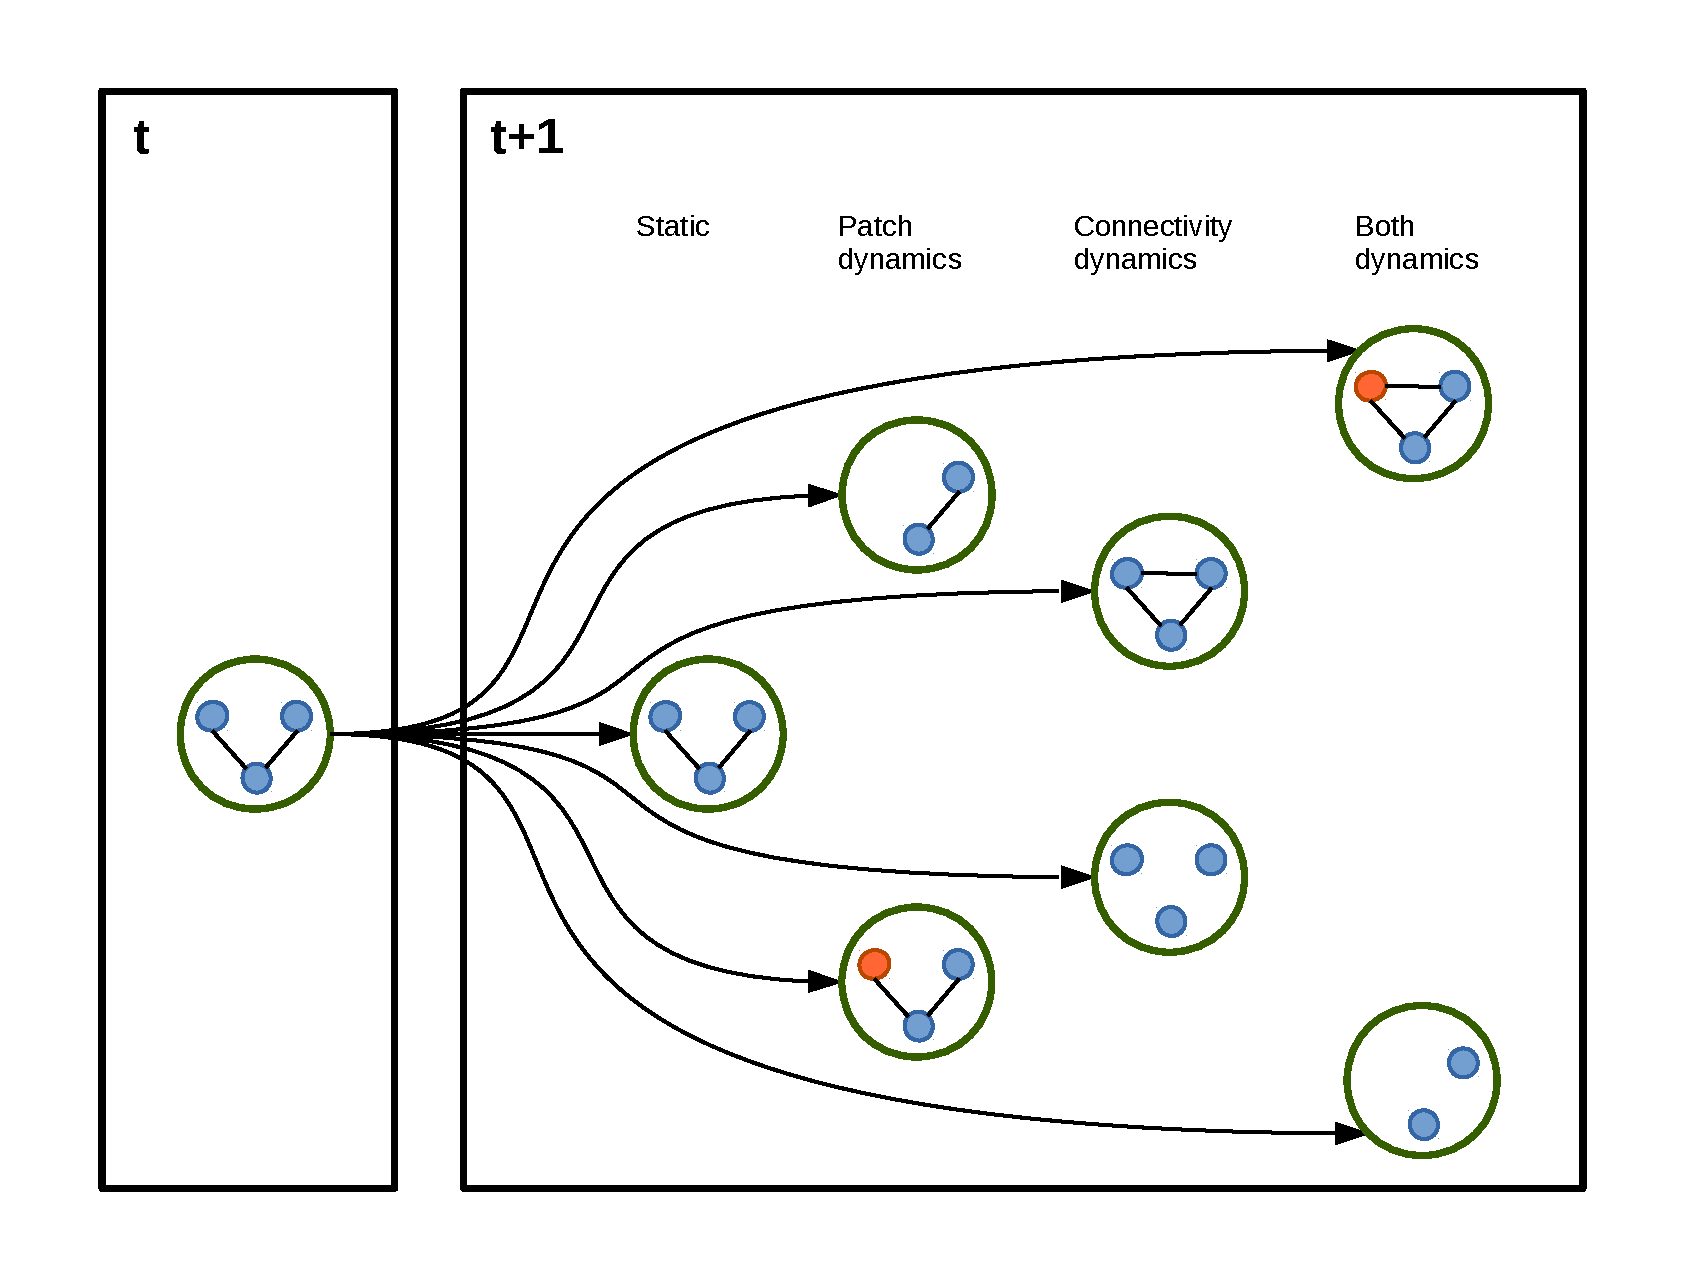
\includegraphics[width=6.75in]{./figures/Figure2.eps}
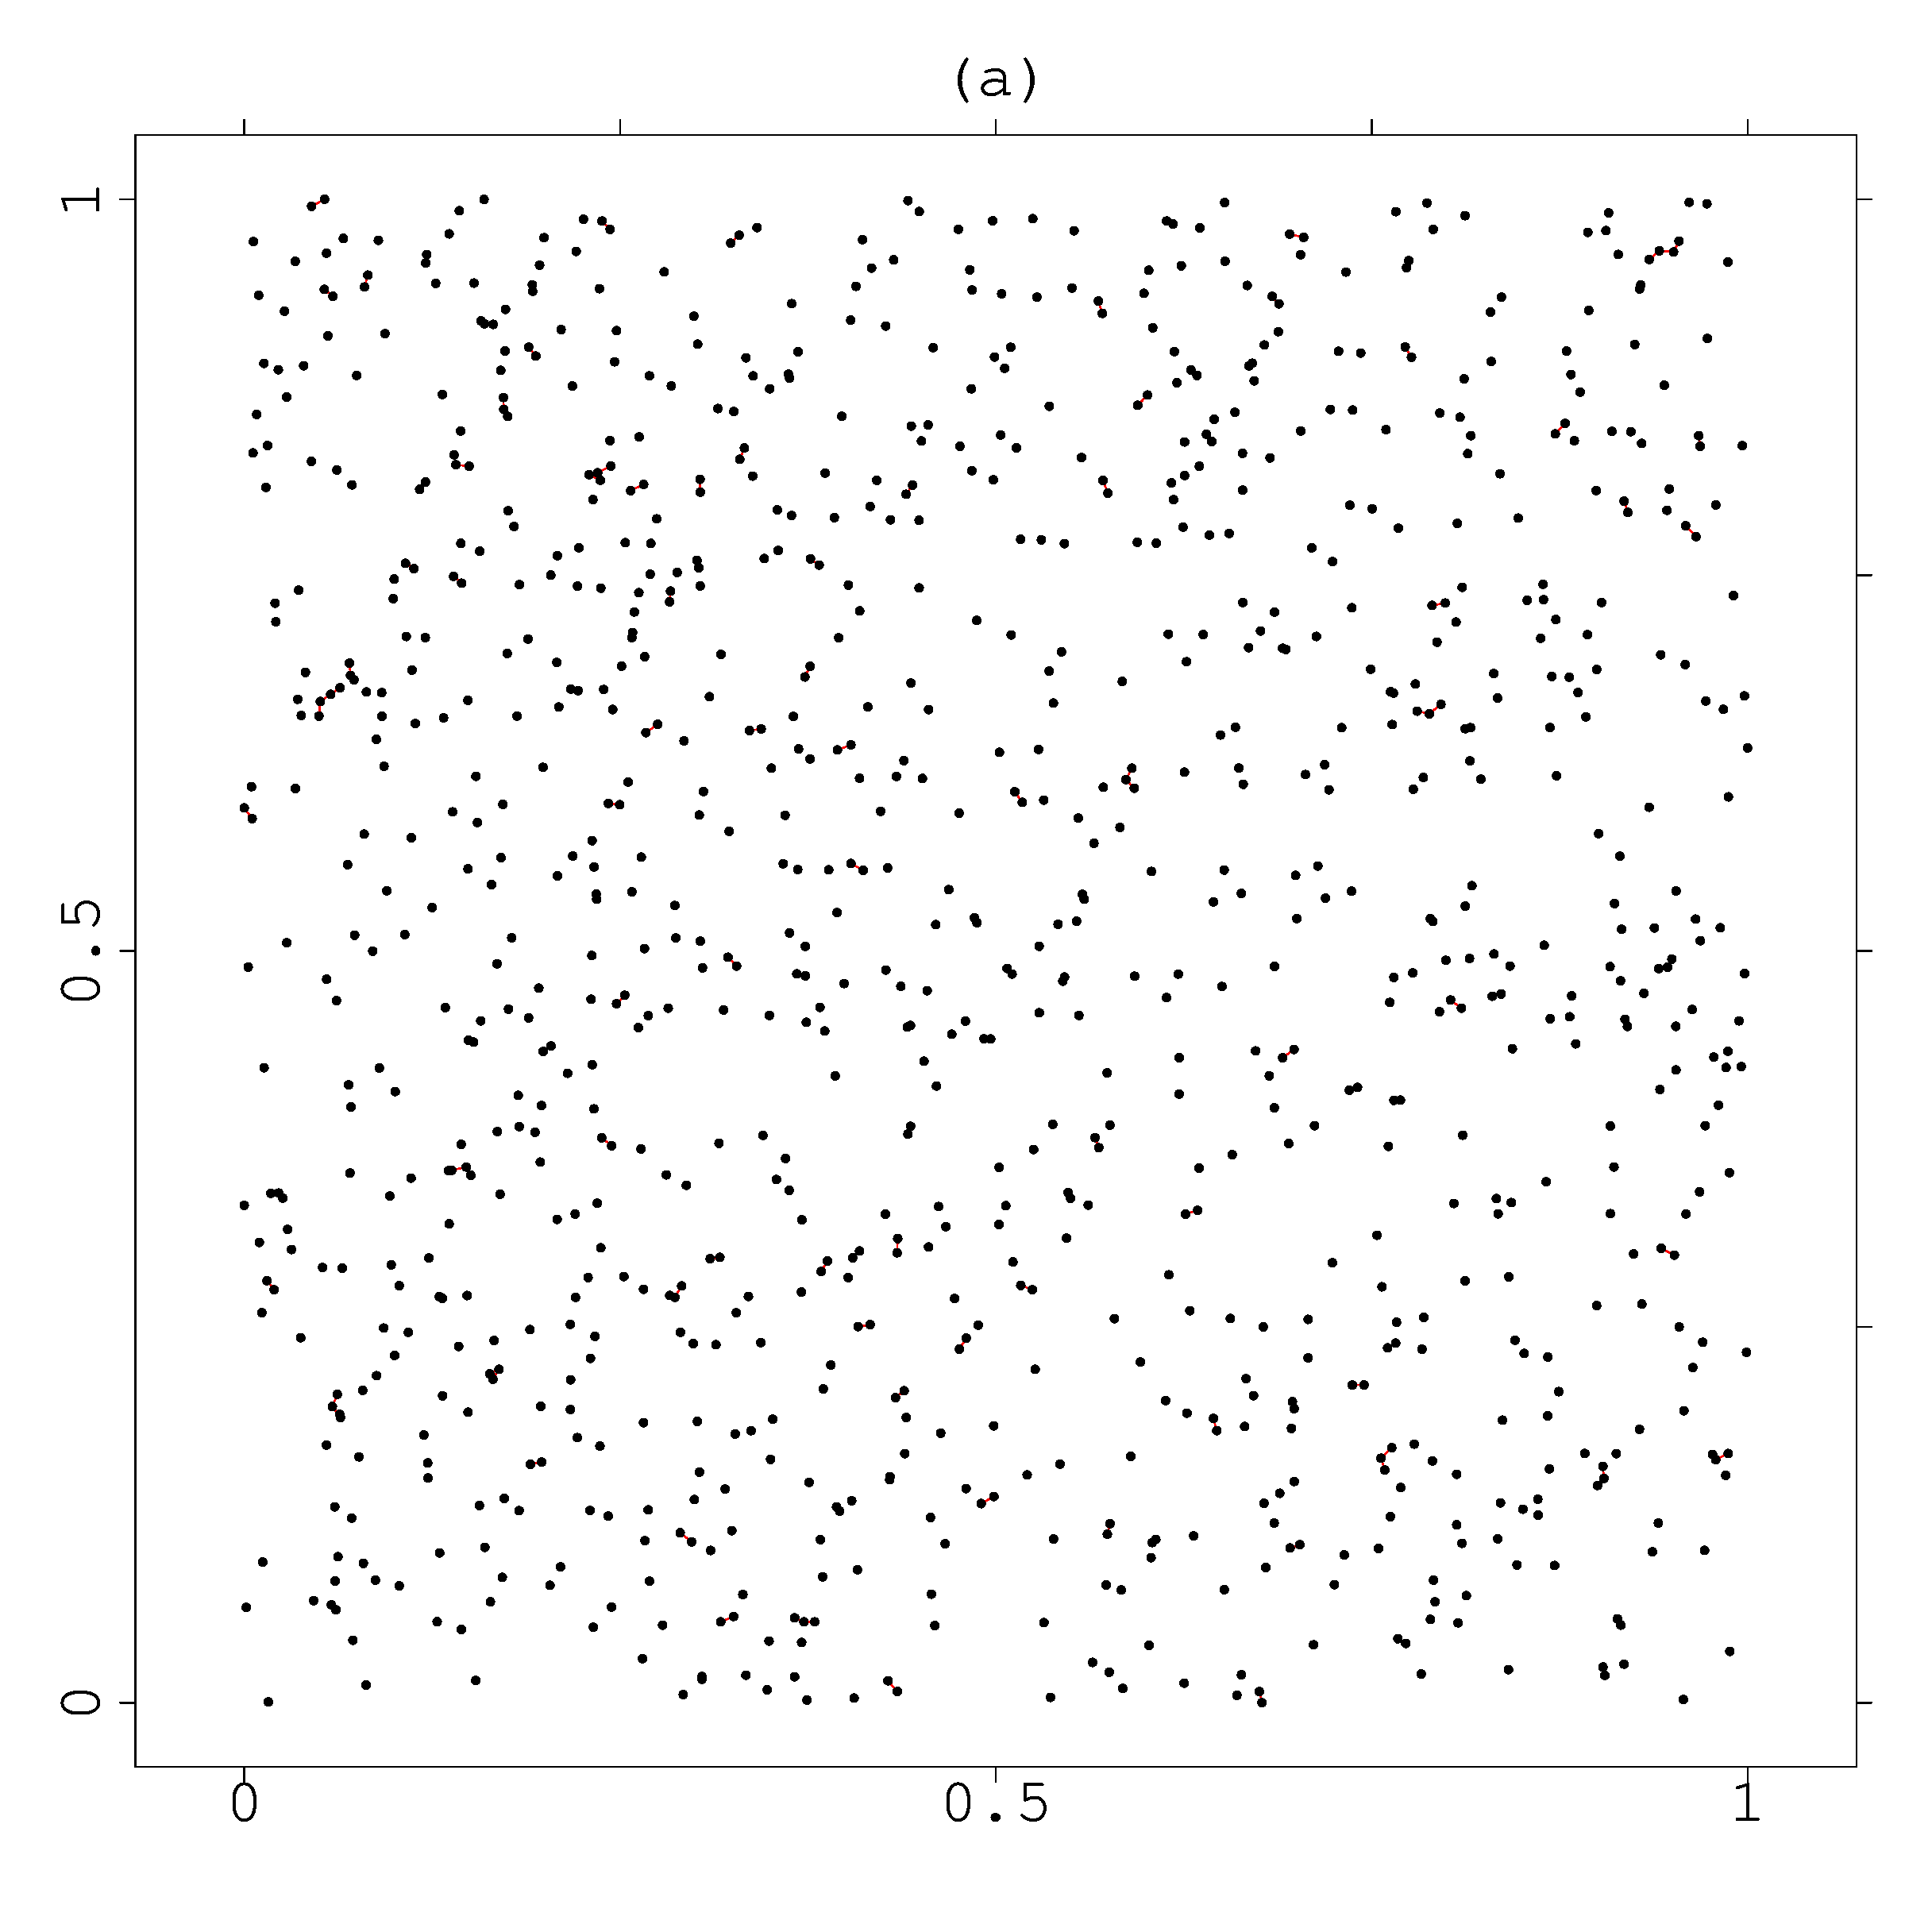
\includegraphics[width=3.1in]{./figures/RGN_r_001.eps}
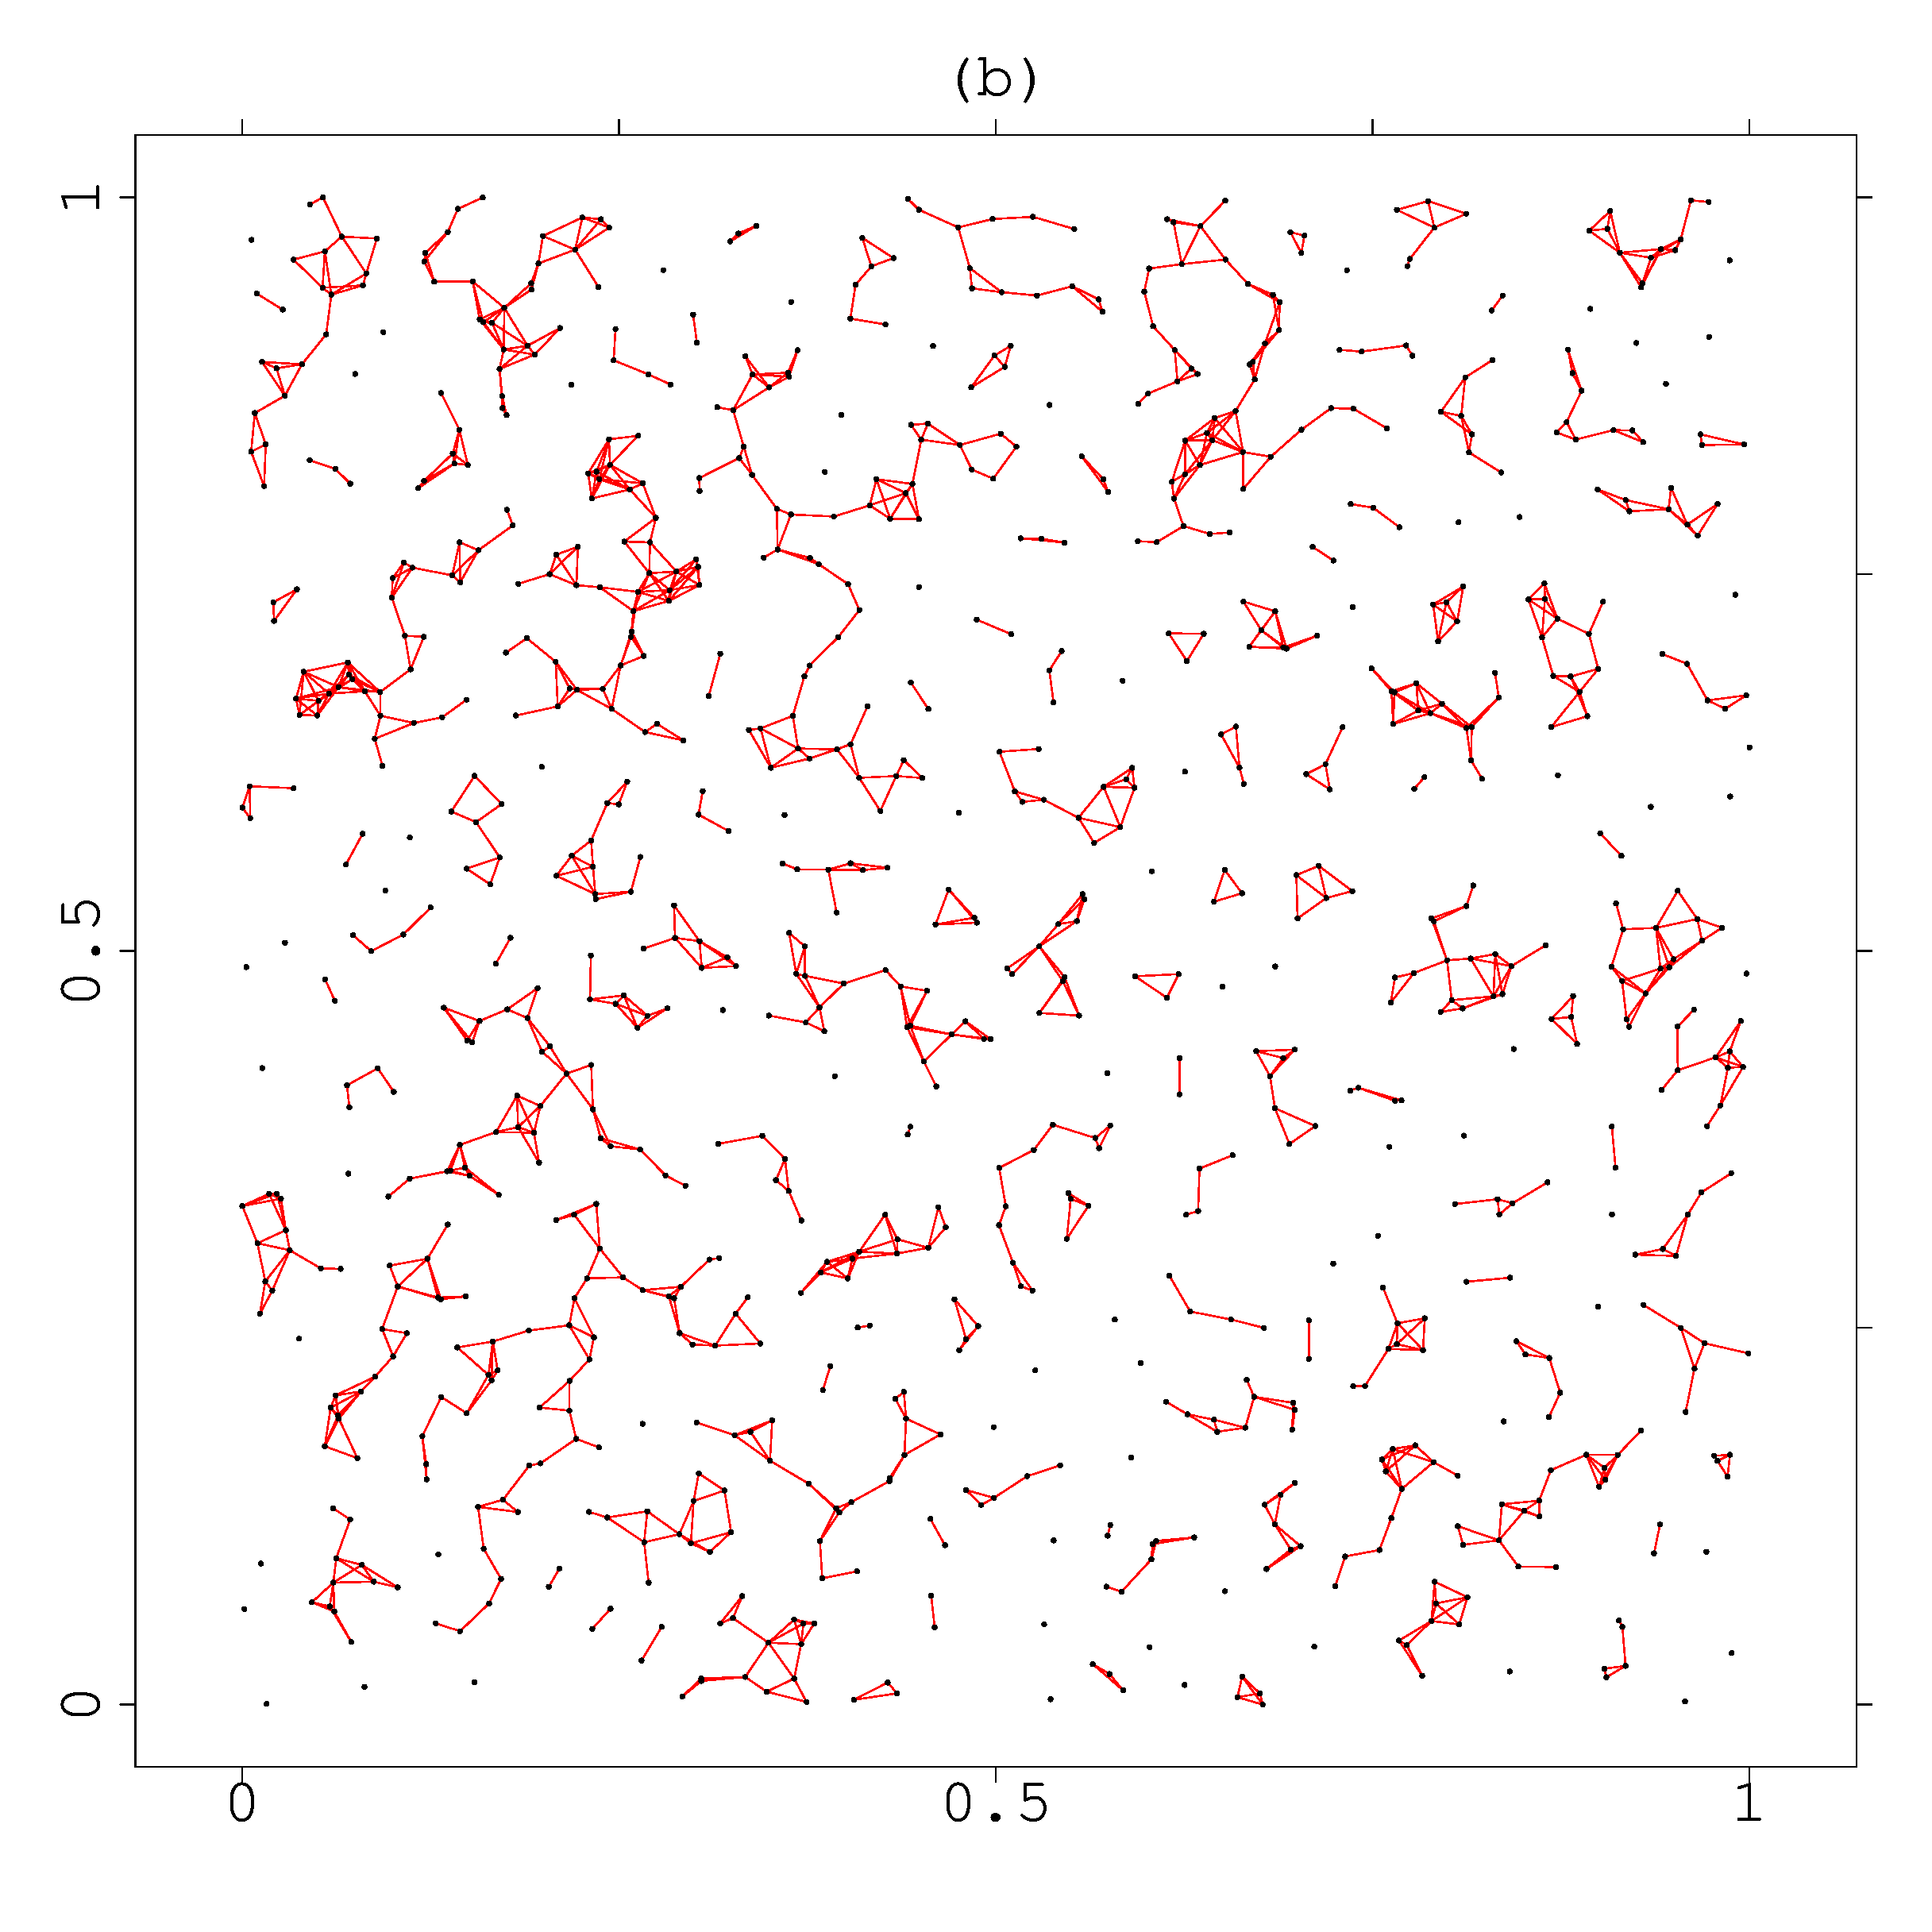
\includegraphics[width=3.1in]{./figures/RGN_r_003.eps}
\includegraphics[width=3.1in]{./figures/RGN_r_0075.eps}
\end{center}
\caption{}
\label{fig:Figure4}
\end{figure}

\begin{figure}[hb!]
\hspace{-0.5 in}\includegraphics[width=5in,angle=-90]{./figures/mean_variance_comp_gamma.eps}
\caption{}
\label{fig:Figure5}
\end{figure}

\begin{figure}[hb!]
\hspace{-0.5 in}\includegraphics[width=5in,angle=-90]{./figures/mean_variance_radius_gamma.eps}
\caption{}
\label{fig:Figure6}
\end{figure}

\begin{figure}[hb!]
\begin{center}
\hspace{-0.5 in}\includegraphics[width=3.5in]{./figures/Figure5.eps}
\end{center}
\caption{}
\label{fig:Figure7}
\end{figure}


\appendix
% Remove brackets from numbering in List of References
\makeatletter
\renewcommand{\@biblabel}[1]{\quad#1.}
\renewcommand{\thefigure}{S\@arabic\c@figure} 
\makeatother
% Leave date blank
%\date{}
\pagestyle{myheadings}
%% ** EDIT HERE **
%% END MACROS SECTION
%\begin{document}
%\newpage

\clearpage
\begin{flushleft} 
{\Large \textbf{Appendix A from C. N. de Santana, J. Klecka, G. M. Palamara, and C. J. Meli\'{a}n, Metacommunities in dynamic landscapes}}
\end{flushleft}
\renewcommand{\theequation}{A-\arabic{equation}}
\setcounter{equation}{0}
\renewcommand{\thesection}{A\arabic{section}}
\renewcommand{\thefigure}{A\arabic{figure}}
\renewcommand{\thetable}{A\arabic{table}}
\setcounter{figure}{0}
\setcounter{table}{0}

\section*{Landscape dynamics animations}
%\vspace{2 in}
SI-A1; Sea Arctic ice cover animation (ArcticSI-A1.flv)
\carlos{CAPTION}
\\
SI-A2; Sea Antarctic ice cover animation (AntarcticSI-A2.flv)
\carlos{CAPTION}
\\
SI-A3; Dynamic landscape animation (RGNSI-A3.ogv)
\carlos{CAPTION}

\clearpage
\begin{flushleft} 
{\Large \textbf{Appendix B from C. N. de Santana, J. Klecka, G. M. Palamara, and C. J. Meli\'{a}n, Metacommunities in dynamic landscapes}}
\end{flushleft}
\renewcommand{\theequation}{B-\arabic{equation}}
\setcounter{equation}{0}
\renewcommand{\thesection}{B\arabic{section}}
\renewcommand{\thefigure}{B\arabic{figure}}
\renewcommand{\thetable}{B\arabic{table}}
\setcounter{figure}{0}
\setcounter{table}{0}

\section*{Metacommunity studies with patch and connectivity dynamics}
\vspace{2 in}
\begin{figure}
\fbox{\parbox[c]{15cm}{
\begin{tabular}{ p{1.5cm} |  p{1.5cm}  |  p{3.5cm}  | p{3.5cm} |  p{3.5cm} | p{3.5cm} }
  \hline
 & & {\textbf{Connectivity}} & & \\ \hline
  \hline                                        
 &   & \textbf{Static}  & \textbf{Random} & \textbf{Seasonal}   \\
  \hline                                        
 & {\textbf{Static}}   & Most studies  & ?  & This paper \\
 &                     &              &     & \cite{GrenfellEtAl1995_seasonality}  \\
&                                    &     &        & \cite{Ross2010}      \\
  \hline                                        
 {\textbf{Habitat}}  & {\textbf{Random}}   & \cite{Hanski1999}   & ?      & ?          \\
 &    & \cite{VuilleumierEtAl2007} &        &            \\
 &    & \cite{DrechslerJohst2010}  &        &            \\
  \hline                                        
& {\textbf{Seasonal}} & \cite{HoltCovlin1997}      & ?      & ?          \\
&                                    & \cite{LoreauEtAl2003}      &        &            \\
  \hline                                        
\end{tabular}
\caption{{\small {\bf Examples of metacommunity or
    metapopulation studies with patch and connectivity
    combinations. Studies included in the category with periodic
    connectivity changes are mostly studies of infectious diseases
    (host-parasite interactions) with seasonal variation in
    transmission rate; see also \cite{FerrariEtAl2008,
      BalcanEtAl2009_seasonal} for examples of applications for
    predicting the spread of diseases. Interrogants mean we are not
    aware of any studies addressing this combination. \carlos{THIS IS PROBABLY THE FIGURE THAT REQUIRES MORE WORK: SHOULD WE MOVE FORWARD IT OR DELETE?}}}}
\label{fig:SI-B1}
}}
\end{figure}


\clearpage
\begin{flushleft} 
{\Large \textbf{Appendix C from C. N. de Santana, J. Klecka, G. M. Palamara, and C. J. Meli\'{a}n, Metacommunities in dynamic landscapes}}
\end{flushleft}

\renewcommand{\theequation}{C-\arabic{equation}}
\setcounter{equation}{0}
\renewcommand{\thesection}{C\arabic{section}}
\renewcommand{\thefigure}{C\arabic{figure}}
\renewcommand{\thetable}{C\arabic{table}}
\setcounter{figure}{0}
\setcounter{table}{0}

\section*{Stochastic metacommunity landscape dynamics}
\label{Population dispersal model}

Here, we explain in detail how we combine dispersal with local
population dynamics. The following equations conceptualize
metacommunity dynamics. The first (second) equation gives the
transition probability that the $k^{th}$ species of
metacommunity declines (increases) in abundance by one individual in
patch $i$
\begin{equation}
\begin{array}{lcr}
\hspace{-0.25 in}P \left(N_{i}^{k} - 1 | N_{i}^{k} \right) = M^{k}_{i} \left[\sum\limits^{\mathcal{P}}_{\substack{j = 1,j \ne i \\ \mathfrak{d_{ij}} \leq \mathfrak{d_{c}}}}
 \sum\limits_{k'=1,k'\ne k}^{S_{j}} m_{ij}^{k'} \left(\frac{N_{j}^{k'}}{J_{j}}\right) + \lambda \left(\frac{J_{i} - N_{i}^{k}}{J_{i} - 1}\right) + \nu \right]\\[0.5cm]
%\label{master1}
\\
\hspace{-0.25 in}P \left(N_{i}^{k} + 1 | N_{i}^{k}\right) = (1 - M^{k}_{i}) \left[
\sum\limits^{\mathcal{P}}_{\substack{j = 1,j \ne i \\ \mathfrak{d_{ij}} \leq \mathfrak{d_{c}}}}
%\sum\limits_{j=1,j\ne i}^{\mathcal{P}}
 m_{ij}^{k} \left(\frac{N_{j}^{k}}{J_{j}}\right) + \lambda \left(\frac{N_{i}^{k}}{J_{i} - 1}\right) + \nu \right].
\end{array}
\label{master}
\end{equation}
Here $M^{k}_{i}$ describes density-dependent mortality rate of species
$k$ in patch $i$. This mortality is the natural per capita mortality
rate described in this article by $\mu
\frac{N_{i}^{k}}{J_{i}}$. $N_{i}^{k}$ and $J_{i}$ are the total number of
individuals of species $k$ in patch $i$ and the number of individuals
in patch $i$, respectively. $\mathcal{S}_{j}$ and $\mathcal{P}$ are
the total number of species in patch $j$ and the total number of
patches, respectively. In addition to the mortality rate parameters,
there are three more metacommunity specific parameters: $\lambda$, the
local birth rate, $m$, the intensity of emigration rate, and $\nu$,
the immigration rate from the regional species pool.

The first equation in (\ref{master}) gives the transition probability
for the $k^{th}$ species to decline in abundance by one individual in
patch $i$. For this to happen, an individual must die in the $k^{th}$
species, which occurs at a rate given by $M^{k}_{i}$. The first
probability inside the brackets is that of an immigration event of
some species other than $k$ from a patch different to $i$ (see
equation 2 in the main text with $\mathfrak{d_{ij}}$ the geographical
distance between patch $i$ and $j$ satisfying $\mathfrak{d_{ij}}$
$\leq$ $\mathfrak{d_{c}}$). The second term represents the probability
of having a local birth in a species other than $k$ with the -1
subtracted in the denominator after the death in the previous step of
one individual in this patch. The third term describes the probability
of an immigration event from the regional species pool. The second
equation in (\ref{master}) describes the transition probability for
the $k^{th}$ species to increase by one individual. For this to
happen, there must be no local death in species $k$ which is given by
$1 - M^{k}_{i}$. The other terms in brackets stand for dispersal (the
first term), local birth of an individual of species $k$ (second
term), and immigration of a new species $k$ from the regional species
pool. This last event can occur only when there was no such species,
i.e., when $N_{i}^{k}$ $=$ 0 at time $t - 1$.  

\clearpage
\begin{flushleft} 
{\Large \textbf{Appendix D from C. N. de Santana, J. Klecka, G. M. Palamara, and C. J. Meli\'{a}n, Metacommunities in dynamic landscapes}}
\section*{Mean $\gamma-$species richness}
\end{flushleft}
\renewcommand{\theequation}{D-\arabic{equation}}
\setcounter{equation}{0}
\renewcommand{\thesection}{D\arabic{section}}
\renewcommand{\thefigure}{D\arabic{figure}}
\renewcommand{\thetable}{D\arabic{table}}
\setcounter{figure}{0}
\setcounter{table}{0}

\begin{figure}[hb!]
\begin{center}

\includegraphics[width=2.2in, angle=-90]{./figures/Figure6_Mean_a_003.eps}\hspace{-0.025 in}
\includegraphics[width=2.2in, angle=-90]{./figures/Figure6_Mean_b_003.eps}\\
\includegraphics[width=2.2in, angle=-90]{./figures/Figure6_Mean_c_003.eps}\hspace{-0.025 in}
\includegraphics[width=2.2in, angle=-90]{./figures/Figure6_Mean_d_003.eps}\\

\end{center}
\caption{This figure shows the mean $\gamma-$species richness as a function of amplitude, $\mathcal{A}$, and frequency, $\mathfrak{f}$, for four landscape metrics. (a) Isoclines values represent the mean landscape connectivity calculated as $2\sum_{i}^{\mathcal{P}} \Gamma_{i}/(\mathcal{P}(\mathcal{P} - 1))$, with $\mathcal{P}$, the total number of patches, and $\Gamma_{i}$, the connectivity of patch $i$. (b) Isoclines values represent the mean number of components, $\hat{\mathcal{C}}$. (c) Isoclines values represent the mean landscape continuity, calculated as ($\mathcal{P} - \mathcal{C}$)/$\mathcal{P}$, with $\mathcal{P}$, the total number of patches, and $\mathcal{C}$ the number of components. (d) Isoclines values represent the mean landscape availability calculated as the ratio between landscape connectivity and landscape continuity. Simulations were done for emigration rate, $\mathrm{m}$ = 0.1, immigration rate from the species regional pool, $\mathrm{\nu}$ = 0.003, total number of patches, $\mathcal{P}$ = 100, patch size, $J_{x_i,y_i}$ = 100 individuals and number of generations per replicate, $\mathcal{G}$ = 1000. $\gamma-$species richness was averaged over the last 500 generations in each replicate.}
\label{fig:SI-D1}
\end{figure}

\clearpage
\begin{flushleft} 
{\Large \textbf{Appendix E from C. N. de Santana, J. Klecka, G. M. Palamara, and C. J. Meli\'{a}n, Metacommunities in dynamic landscapes}}
\section*{Mean $\gamma-$species richness and landscape metrics}
\end{flushleft}
\renewcommand{\theequation}{E-\arabic{equation}}
\setcounter{equation}{0}
\renewcommand{\thesection}{E\arabic{section}}
\renewcommand{\thefigure}{E\arabic{figure}}
\renewcommand{\thetable}{E\arabic{table}}
\setcounter{figure}{0}
\setcounter{table}{0}

\begin{figure}[hb!]
\begin{center}
%\begin{tabular}{cc}
\includegraphics[width=2.5in]{./figures/new_A_r0_MeanGamma_001.eps}\hspace{-0.025 in}
\includegraphics[width=2.5in]{./figures/new_A_r0_MeanGamma_004.eps}\\
\includegraphics[width=2.5in]{./figures/new_A_r0_MeanGamma_007.eps}\hspace{-0.025 in}
\includegraphics[width=2.5in]{./figures/new_A_r0_MeanGamma_010.eps}\\
%\end{tabular}
\end{center}
\caption{This figure shows the mean $\gamma-$species
    richness as a function the dispersal radius, $\mathfrak{d_{c}}$), and amplitude, $\mathcal{A}$, for static
    (black, $\mathcal{A}$ = 0), coupled dynamic (blue, $\mathcal{A}$ =
    $\mathfrak{d_{0}}$), and dynamic landscapes (red, $\mathcal{A}$ =
    1) for four frequency, $\mathfrak{f}$, values, (a) $0.001$, (b)
    $0.01$, (c) $0.1$ , and (d) $1$. Vertical dotted line represents
    the critical threshold in static landscapes. Isoclines
    (dotted lines) represent the mean number of components,
    $\hat{\mathcal{C}}$, for each combination of dispersal radius,
    $\mathfrak{d_{c}}$, and amplitude $\mathcal{A}$. Simulations were
    done for emigration rate, $\mathrm{m}$ = 0.1, immigration rate
    from the species regional pool, $\mathrm{\nu}$ = 0.003, total
    number of patches, $\mathcal{P}$ = 100, patch size, $J_{x_i,y_i}$
    = 100 individuals and number of generations per replicate,
    $\mathcal{G}$ = 1000. Values plotted represent the mean values
    over the last 500 generations in each replicate.}
\label{fig:SI-E1}
\end{figure}
\end{document}

